%4619055 課題3 パルス回路
\documentclass[12pt]{jarticle}
\usepackage{TUSIreport}
\usepackage{otf}
\usepackage[dvipdfmx]{graphicx}
\usepackage{amsmath}
\usepackage{amssymb}
\usepackage{hhline}
\usepackage{fancybox,ascmac}
\usepackage{url}
%%%%%%%%%%%%%%%%%%
\begin{document}
%%%%%%%%%%%%%%%%%%%%%%%%%%%%%%%%%%%%%%%%%%%%%%%%%%%%%%%%
% 表紙を出力する場合は,\提出者と\共同実験者をいれる
% \提出者{科目名}{課題名}{提出年}{提出月}{提出日}{学籍番号}{氏名}
% \共同実験者{一人目}{二人目}{..}{..}{..}{..}{..}{八人目}
%%%%%%%%%%%%%%%%%%%%%%%%%%%%%%%%%%%%%%%%%%%%%%%%%%%%%%%
\提出者{情報工学実験1}{課題4 統計学入門}
{2020}{7}{27}{4619055}{辰川力駆}

\共同実験者{}{}{}{}{}{}{}{}
\追加実験者{}{}
\表紙出力

\section{実験の目的}
実験を通して、誤差を体感し、データを視覚的に表現する

\section{実験1}
サイコロを用いたギャンブル

\subsection{目標}
\begin{itemize}
    \item 実験を通して実際にデータがばらつくことを実感する
    \item 簡単なギャンブルを例に、誤差について考える
\end{itemize}
\subsection{実験手順}
\begin{itemize}
    \item[(1)] 1回の試行でサイコロ(出る目は0から9)を2個同時に振り、
          出た目の合計で以下のように収支が決まるギャンブルを考える
          \begin{itemize}
              \item 合計が7以下・・・1000円払う
              \item 合計が12以上・・・1500円もらう
              \item それ以外・・・引き分け
          \end{itemize}
    \item[(2)] 試行を100回繰り返し、各試行の目の合計・収支を記録する
    \item[(3)] 試行回数5回ごとに、1回目からの平均収支を求める
    \item[(4)] 横軸に試行回数、縦軸に1回目からの平均収支をとり、
          平均収支が収束する様子をグラフで表現する(期待収支も記入)
\end{itemize}
\subsection{実験結果と考察}
以下にサイコロを100回振った結果と、サイコロを用いたギャンブルによる平均収支のグラフを示す。

\clearpage
\begin{table}
    \caption{サイコロを用いたギャンブルの記録}
    \begin{tabular}[h]{|r|c|c|c|c|c|c|}
        \hline
        試行回数 & サイコロ1の目 & サイコロ2の目 & 出た目の合計 & 収支  & 試行回数 & 平均収支     \\ \hline
        1        & 6             & 9             & 15           & 1500  &          &              \\
        2        & 8             & 7             & 15           & 1500  &          &              \\
        3        & 0             & 5             & 5            & -1000 & 5        & 200          \\
        4        & 4             & 6             & 10           & 0     &          &              \\
        5        & 7             & 0             & 7            & -1000 &          &              \\
        \hline6  & 6             & 3             & 9            & 0     &          &              \\
        7        & 5             & 2             & 7            & -1000 &          &              \\
        8        & 2             & 6             & 8            & 0     & 10       & 150          \\
        9        & 8             & 2             & 10           & 0     &          &              \\
        10       & 8             & 5             & 13           & 1500  &          &              \\
        \hline11 & 0             & 8             & 8            & 0     &          &              \\
        12       & 9             & 6             & 15           & 1500  &          &              \\
        13       & 4             & 6             & 10           & 0     & 15       & 66.66666667  \\
        14       & 5             & 1             & 6            & -1000 &          &              \\
        15       & 2             & 0             & 2            & -1000 &          &              \\
        \hline16 & 1             & 2             & 3            & -1000 &          &              \\
        17       & 9             & 1             & 10           & 0     &          &              \\
        18       & 7             & 3             & 10           & 0     & 20       & 0            \\
        19       & 4             & 6             & 10           & 0     &          &              \\
        20       & 0             & 9             & 9            & 0     &          &              \\
        \hline21 & 7             & 9             & 16           & 1500  &          &              \\
        22       & 4             & 1             & 5            & -1000 &          &              \\
        23       & 1             & 4             & 5            & -1000 & 25       & -20          \\
        24       & 7             & 1             & 8            & 0     &          &              \\
        25       & 4             & 6             & 10           & 0     &          &              \\
        \hline26 & 3             & 4             & 7            & -1000 &          &              \\
        27       & 2             & 9             & 11           & 0     &          &              \\
        28       & 6             & 1             & 7            & -1000 & 30       & -66.66666667 \\
        29       & 3             & 9             & 12           & 1500  &          &              \\
        30       & 6             & 0             & 6            & -1000 &          &              \\
        \hline31 & 5             & 9             & 14           & 1500  &          &              \\
        32       & 7             & 6             & 13           & 1500  &          &              \\
        33       & 4             & 6             & 10           & 0     & 35       & 71.42857143  \\
        34       & 8             & 6             & 14           & 1500  &          &              \\
        35       & 3             & 8             & 11           & 0     &          &              \\
        \hline36 & 6             & 6             & 12           & 1500  &          &              \\
        37       & 5             & 6             & 11           & 0     &          &              \\
        38       & 0             & 7             & 7            & -1000 & 40       & 50           \\
        39       & 8             & 0             & 8            & 0     &          &              \\
        40       & 6             & 1             & 7            & -1000 &          &              \\
        \hline
    \end{tabular}
\end{table}
\clearpage
\begin{table}
    \begin{tabular}[h]{|r|c|c|c|c|c|c|}
        \hline
        試行回数  & サイコロ1の目 & サイコロ2の目 & 出た目の合計 & 収支  & 試行回数 & 平均収支    \\ \hline
        41        & 9             & 0             & 9            & 0     &          &             \\
        42        & 7             & 2             & 9            & 0     &          &             \\
        43        & 7             & 4             & 11           & 0     & 45       & 77.77777778 \\
        44        & 8             & 9             & 17           & 1500  &          &             \\
        45        & 2             & 8             & 10           & 0     &          &             \\
        \hline 46 & 4             & 2             & 6            & -1000 &          &             \\
        47        & 5             & 4             & 9            & 0     &          &             \\
        48        & 3             & 9             & 12           & 1500  & 50       & 80          \\
        49        & 3             & 5             & 8            & 0     &          &             \\
        50        & 8             & 2             & 10           & 0     &          &             \\
        \hline 51 & 1             & 1             & 2            & -1000 &          &             \\
        52        & 9             & 4             & 13           & 1500  &          &             \\
        53        & 9             & 8             & 17           & 1500  & 55       & 109.0909091 \\
        54        & 4             & 5             & 9            & 0     &          &             \\
        55        & 1             & 7             & 8            & 0     &          &             \\
        \hline 56 & 0             & 3             & 3            & -1000 &          &             \\
        57        & 9             & 3             & 12           & 1500  &          &             \\
        58        & 1             & 3             & 4            & -1000 & 60       & 91.66666667 \\
        59        & 4             & 6             & 10           & 0     &          &             \\
        60        & 5             & 6             & 11           & 0     &          &             \\
        \hline 61 & 0             & 0             & 0            & -1000 &          &             \\
        62        & 1             & 2             & 3            & -1000 &          &             \\
        63        & 5             & 3             & 8            & 0     & 65       & 23.07692308 \\
        64        & 4             & 0             & 4            & -1000 &          &             \\
        65        & 6             & 0             & 6            & -1000 &          &             \\
        \hline66  & 3             & 8             & 11           & 0     &          &             \\
        67        & 8             & 2             & 10           & 0     &          &             \\
        68        & 7             & 8             & 15           & 1500  & 70       & 28.57142857 \\
        69        & 8             & 1             & 9            & 0     &          &             \\
        70        & 3             & 1             & 4            & -1000 &          &             \\
        \hline71  & 7             & 4             & 11           & 0     &          &             \\
        72        & 3             & 2             & 5            & -1000 &          &             \\
        73        & 2             & 3             & 5            & -1000 & 75       & 20          \\
        74        & 9             & 8             & 17           & 1500  &          &             \\
        75        & 6             & 5             & 11           & 0     &          &             \\
        \hline76  & 5             & 2             & 7            & -1000 &          &             \\
        77        & 6             & 7             & 13           & 1500  &          &             \\
        78        & 0             & 1             & 1            & -1000 & 80       & -12.5       \\
        79        & 4             & 0             & 4            & -1000 &          &             \\
        80        & 1             & 1             & 2            & -1000 &          &             \\
        \hline
    \end{tabular}
\end{table}
\clearpage
\begin{table}
    \begin{tabular}[h]{|r|c|c|c|c|c|c|}
        \hline
        試行回数 & サイコロ1の目 & サイコロ2の目 & 出た目の合計 & 収支  & 試行回数 & 平均収支     \\
        \hline
        81       & 6             & 5             & 11           & 0     &          &              \\
        82       & 4             & 6             & 10           & 0     &          &              \\
        83       & 3             & 3             & 6            & -1000 & 85       & -5.882352941 \\
        84       & 2             & 6             & 8            & 0     &          &              \\
        85       & 5             & 7             & 12           & 1500  &          &              \\
        \hline
        86       & 4             & 3             & 7            & -1000 &          &              \\
        87       & 9             & 0             & 9            & 0     &          &              \\
        88       & 4             & 8             & 12           & 1500  & 90       & -22.22222222 \\
        89       & 0             & 0             & 0            & -1000 &          &              \\
        90       & 0             & 6             & 6            & -1000 &          &              \\
        \hline
        91       & 4             & 8             & 12           & 1500  &          &              \\
        92       & 7             & 5             & 12           & 1500  &          &              \\
        93       & 2             & 8             & 10           & 0     & 95       & -10.52631579 \\
        94       & 0             & 6             & 6            & -1000 &          &              \\
        95       & 3             & 4             & 7            & -1000 &          &              \\
        \hline
        96       & 0             & 9             & 9            & 0     &          &              \\
        97       & 3             & 1             & 4            & -1000 &          &              \\
        98       & 7             & 8             & 15           & 1500  & 100      & -15          \\
        99       & 1             & 0             & 1            & -1000 &          &              \\
        100      & 7             & 2             & 9            & 0     &          &              \\
        \hline
    \end{tabular}
\end{table}
\begin{figure}[h]
    \begin{center}
        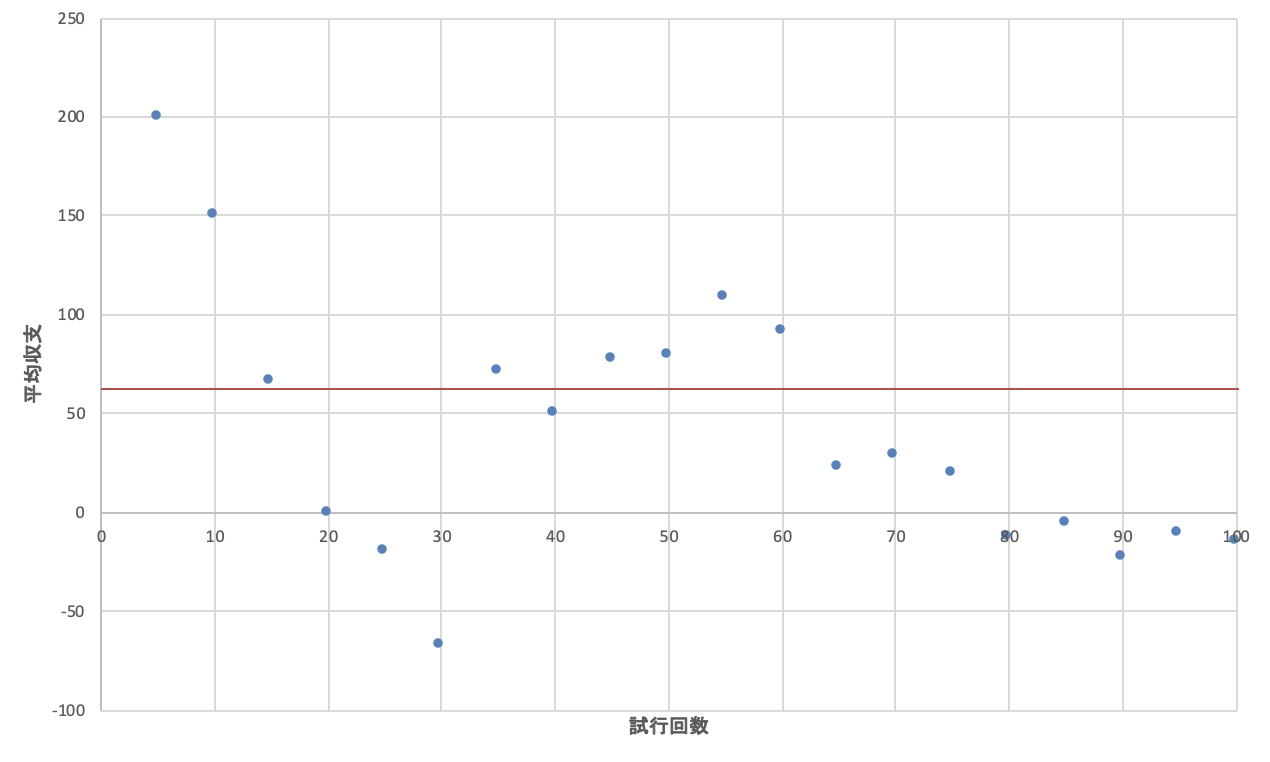
\includegraphics[scale=0.8]{kadai4_graph1.png}
    \end{center}
    \caption{平均収支の変化}
    \label{fig1}
\end{figure}
\clearpage

また、図1の赤い直線は期待収支を表している。
求め方は、
\begin{eqnarray}
    E[Y] &=& \frac{36}{100}×(-1000) + \frac{28}{100}×1500 + \frac{36}{100}×0 \nonumber\\
    &=& 60
\end{eqnarray}
で求められる。

よって、1 回の収支の期待収支は 60 円と言うことが分かるので、$y(平均収支)=60$の直線を引いている。

\subsection{レポート課題}
\subsubsection*{レポート課題1-1}
\begin{shadebox}
    1回の試行における収支の期待値を計算し、
    5回の試行が終わったときの実験結果と比較せよ。
    さらに、100回の試行が終わったときの実験結果と比較せよ。
\end{shadebox}
式(1)より、1回の試行における収支の期待値は60円である。
これをもとに比較する。

5回の試行が終わったときの平均収支は表1より200円で、
1回の試行における収支の期待値との差は140円となり、差が大きかった。
試行回数が少ないとばらつきが大きくなった。
また、100回の試行が終わったときの平均収支は表1より-15円だった。
1 回の試行における収支の期待値との差は75 円となり、
5 回の試行の結果よりは差が小さかった。
試行回数が増えるとばらつきが減っていくことがわかった。

\subsubsection*{レポート課題1-2}
\begin{shadebox}
    出た目の合計Xのヒストグラムを作成し、
    ヒストグラムからわかることをまとめよ。
\end{shadebox}
出た目の合計 X のヒストグラムは以下の図2ようになる。

図2より中央の値である 7から11辺りが他の値に比べて高くなっている。
これは、今回のサイコロは 0 から 9 まで出るものであるから、
和が 9 になる組み合わせは 10 通りある。
また、8や10もそれには劣るが 9 通りある。
したがって、実験する回数が多くなるほど理論値通りの形に近づき左右対称で山なりな概形になると考える。


今回のヒストグラムは100回しか行わなかったので理論値通りのきれいな形をしていないが、
前述の通り回数を増やせば山なりの概形になると考える。

\clearpage
\begin{figure}[h]
    \begin{center}
        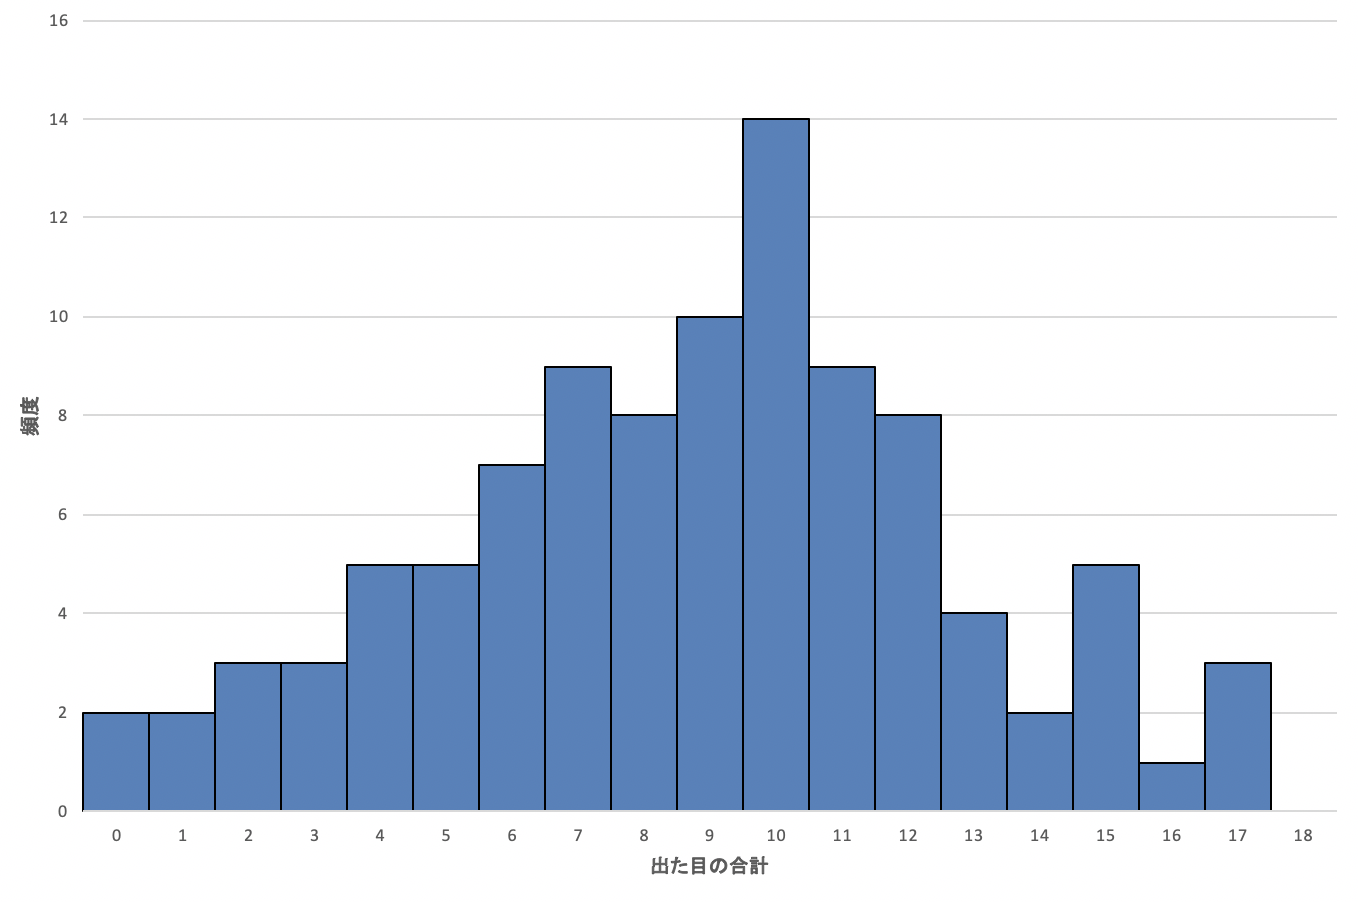
\includegraphics[scale=0.7]{kadai4_graph2.png}
    \end{center}
    \caption{出た目の合計のヒストグラム}
    \label{fig2}
\end{figure}

\subsubsection*{レポート課題1-3}
\begin{shadebox}
    このギャンブルの1回の参加費が120円のとき、
    参加すべきかどうかを理由とともに説明せよ。
    また、サイコロの目が12以上のときに何円受け取ることができればよいか
    (すなわち、期待される収支が0円以上となるか)を述べよ。
\end{shadebox}

今回の1回における期待収支は60円なので1回に120を払っていたら期待値は
\begin{eqnarray}
    60 - 120 = -60 \nonumber
\end{eqnarray}
となりマイナスになる。
したがって、参加するべきではないと考える。

期待される収支が0円以上になるには、
\begin{eqnarray}
    E[Y] &\geq& 120
\end{eqnarray}
すなわち
\begin{eqnarray}
    \frac{36}{100}×(-1000) + \frac{28}{100}×x + \frac{36}{100}×0 &\geq& 120 \nonumber\\
\end{eqnarray}
となれば良い。
これを整数の範囲で解くと、$x\geq1715$となる。
よって1715円以上のとき期待される収支が0円以上となる。
\clearpage


\section{実験2}
データの要約と視覚的表現

\subsection{目標}
\begin{itemize}
    \item データを視覚的に表現する方法を理解する
    \item データの正しい要約を行う
\end{itemize}

\subsection{実験手順}
\begin{itemize}
    \item[(1)] 年収データの平均値・中央値・最頻値を求める
    \item[(2)] 年収を50万円刻みで区切ったヒストグラムを作成する
    \item[(3)] 箱ひげ図を作成する
\end{itemize}

\subsection{実験結果と考察}
下記に、年収データと50 万円刻みで区切ったヒストグラムと箱ひげ図を示す。

年収データにおいて平均値は472.9 万円、中央値は430 万円、最頻値は410万円と420万円となった。
また、下側四部位数は390万円、上側四部位数は500 万円、四部位範囲は110 万円となった。

作成したヒストグラムと箱ひげ図から分かるように、
年収が高い人は平均値の何倍もの値になっており、飛び抜けて高い値となっている。
また、箱ひげ図から外れ値が多いことも読み取れる。
これらのことから、年収が高い人が平均値をたくさんあげているから平均年収が高くなっていると言える。
\clearpage
\begin{table}
    \begin{center}
        \caption{年収データ}
        \begin{tabular}[h!]{|c|c||c|c||c|c||c|c||c|c|}
            \hline
            番号 & 年収 & 番号 & 年収 & 番号 & 年収 & 番号 & 年収 & 番号 & 年収 \\
            \hline
            1    & 120  & 21   & 370  & 41   & 420  & 61   & 460  & 81   & 530  \\
            \hline
            2    & 150  & 22   & 370  & 42   & 420  & 62   & 460  & 82   & 540  \\
            \hline
            3    & 200  & 23   & 380  & 43   & 420  & 63   & 460  & 83   & 540  \\
            \hline
            4    & 200  & 24   & 380  & 44   & 420  & 64   & 460  & 84   & 540  \\
            \hline
            5    & 240  & 25   & 390  & 45   & 420  & 65   & 470  & 85   & 550  \\
            \hline
            6    & 250  & 26   & 390  & 46   & 420  & 66   & 470  & 86   & 580  \\
            \hline
            7    & 250  & 27   & 390  & 47   & 420  & 67   & 480  & 87   & 600  \\
            \hline
            8    & 270  & 28   & 400  & 48   & 420  & 68   & 480  & 88   & 610  \\
            \hline
            9    & 310  & 29   & 400  & 49   & 420  & 69   & 480  & 89   & 640  \\
            \hline
            10   & 320  & 30   & 400  & 50   & 430  & 70   & 480  & 90   & 670  \\
            \hline
            11   & 330  & 31   & 400  & 51   & 430  & 71   & 490  & 91   & 680  \\
            \hline
            12   & 340  & 32   & 410  & 52   & 430  & 72   & 500  & 92   & 690  \\
            \hline
            13   & 340  & 33   & 410  & 53   & 440  & 73   & 500  & 93   & 690  \\
            \hline
            14   & 350  & 34   & 410  & 54   & 440  & 74   & 500  & 94   & 700  \\
            \hline
            15   & 350  & 35   & 410  & 55   & 440  & 75   & 500  & 95   & 850  \\
            \hline
            16   & 350  & 36   & 410  & 56   & 440  & 76   & 500  & 96   & 870  \\
            \hline
            17   & 360  & 37   & 410  & 57   & 440  & 77   & 510  & 97   & 900  \\
            \hline
            18   & 360  & 38   & 410  & 58   & 450  & 78   & 510  & 98   & 1000 \\
            \hline
            19   & 360  & 39   & 410  & 59   & 450  & 79   & 520  & 99   & 1400 \\
            \hline
            20   & 370  & 40   & 410  & 60   & 450  & 80   & 530  & 100  & 1550 \\
            \hline
        \end{tabular}
    \end{center}
\end{table}

\begin{figure}[h]
    \begin{center}
        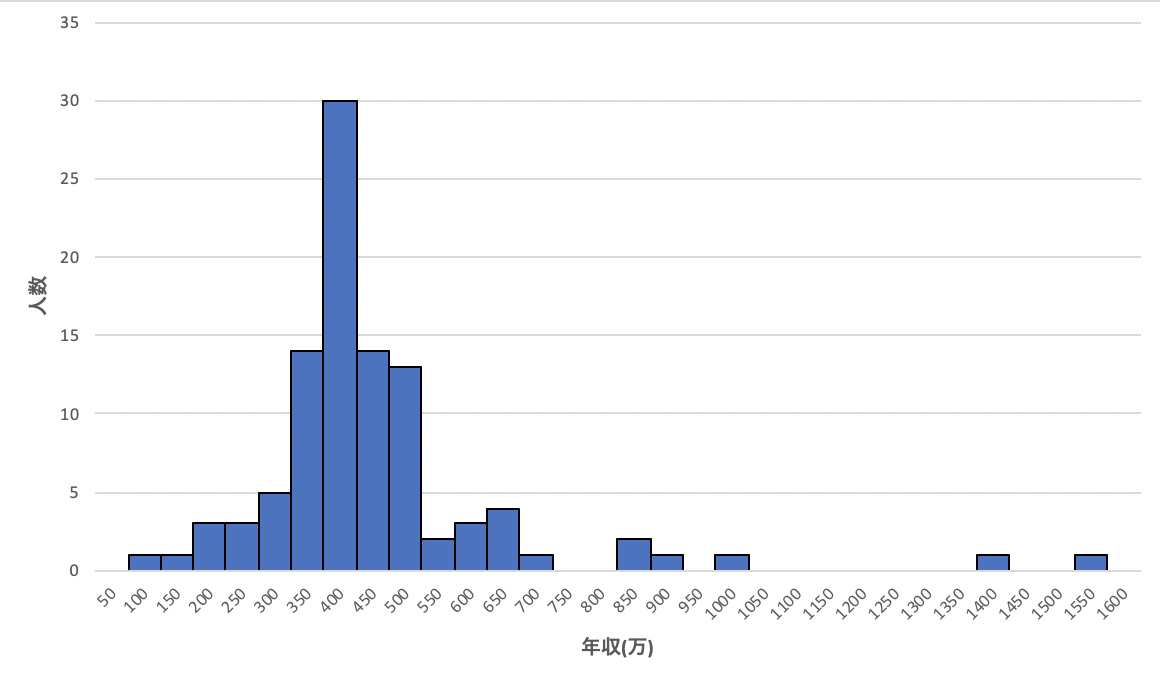
\includegraphics[scale=0.7]{kadai4_graph3.png}
    \end{center}
    \caption{50万円刻みで区切った年収のヒストグラム}
    \label{fig3}
\end{figure}
\clearpage

\begin{figure}[t]
    \begin{center}
        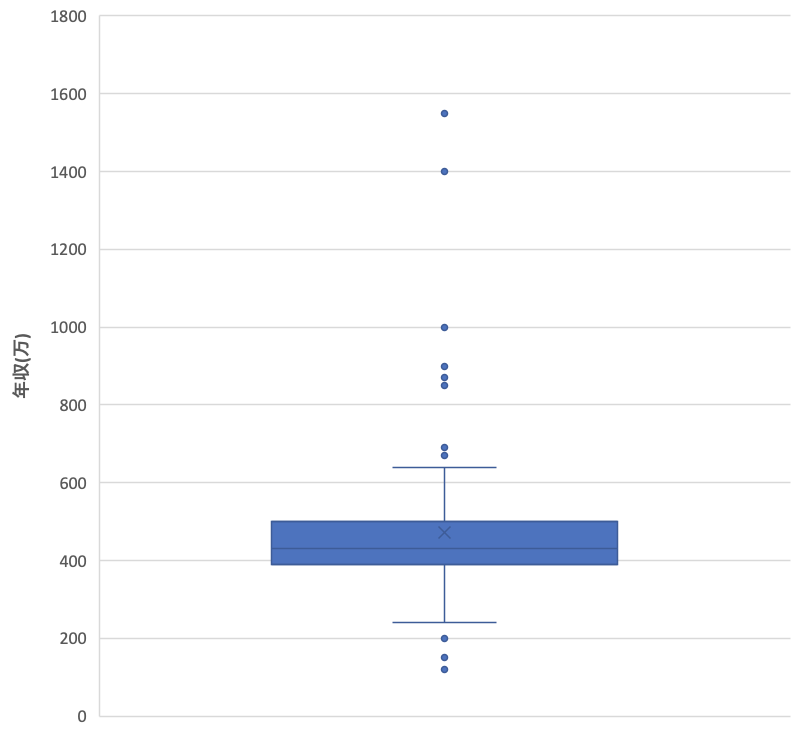
\includegraphics[scale=0.7]{kadai4_graph4.png}
    \end{center}
    \caption{年収の箱ひげ図}
    \label{fig4}
\end{figure}
\subsection{レポート課題}
\subsubsection*{レポート課題2-1}
\begin{shadebox}
    実験2で扱ったデータを用いて2倍の区間幅(100万円刻み)を持つ
    ヒストグラムを作成せよ。
\end{shadebox}

\begin{figure}[h]
    \begin{center}
        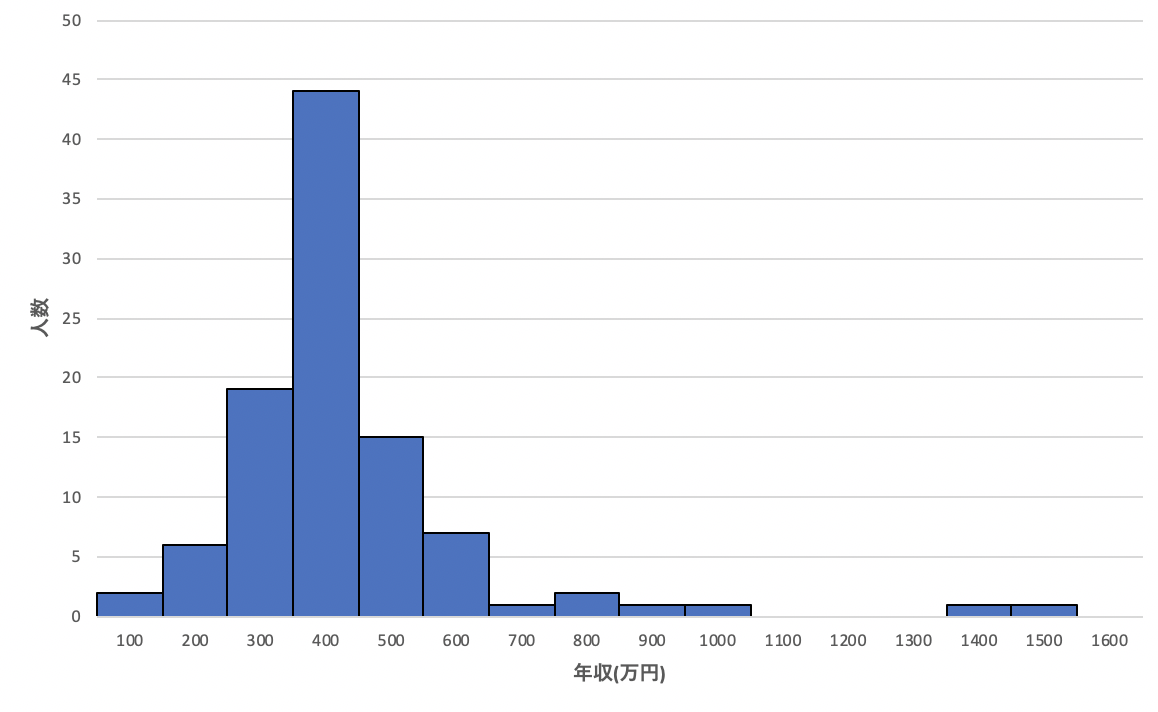
\includegraphics[scale=0.52]{kadai4_graph5.png}
    \end{center}
    \caption{100万円刻みで区切った年収のヒストグラム}
    \label{fig5}
\end{figure}

年収を100万円刻みで区切ったヒストグラムは図5のようになる。

\clearpage
\subsubsection*{レポート課題2-2}
\begin{shadebox}
    作成した2つのヒストグラムを比較し、
    視覚的に得られる情報にどのような違いがあるか考察せよ。
\end{shadebox}

50万円と100万円刻みのヒストグラムの概形には違いはあまりないが、
100万円刻みのヒストグラムから400万円が100人の内ほぼ半分を占めていることが分かる。
また、50万円刻みのヒストグラムの方が細かいので具体的にどこが多いのかが分かりやすい。

データが散らばっている場合は、
ヒストグラムの区間幅を大きくするとデータを扱いやすくなり概形を捉えやすいが、
今回のようにデータがあまり散らばっていない場合は、
ヒストグラムの区間幅を大きくすると細かいデータが分からなくなるので、
区間幅を小さくする方がいいと考える。

\subsubsection*{レポート課題2-3}
\begin{shadebox}
    本データを要約する際に、平均値は適切であるといえるか、理由とともに述べよ。
\end{shadebox}

本データを要約する際に、平均値は適切でないと考える。
理由は、平均値は472.9万円、中央値は430万円、最頻値は410万円と420万円ということに注目すると、
中央値が平均値を大幅に下回っている。
つまり、実験結果でも述べたが数人の高収入の外れ値が平均値を大幅にあげている。

このことから、本データを要約する際に、
平均値だけでなく中央値やヒストグラムなども必要である。

\subsubsection*{レポート課題2-4}
\begin{shadebox}
    ヒストグラムからわかることと、箱ひげ図からわかることの違いを述べよ。
    またそれはなぜかを述べよ。
    さらに、ヒストグラムよりも箱ひげ図を用いたほうが適切だと思われる例を挙げよ。
\end{shadebox}

ヒストグラムは指定範囲のデータの個数が分かるので、
データの分布が分かる。一方、箱ひげ図は外れ値のデータが分かり、
なおかつ平均値や中央値などの値が分かる。

ヒストグラムよりも箱ひげ図を用いたほうが適切だと思われる例としては、
今回のようなデータがあまり散らばっていない場合に有効である。
また、複数のデータ(年収データの場合は2019年と2020年など)の箱ひげ図を並べることで比較することができる。

\clearpage
\subsubsection*{レポート課題2-5}
\begin{shadebox}
    データを要約する指標を列挙し、それぞれの内容と特徴を述べよ。
\end{shadebox}

\begin{itemize}
    \item 平均値

          データの値の合計をデータの数で割ったものであり、
          前述の通り外れ値があると平均値の値が大きくずれるのでこれだけではデータの性質が分からないことがある。
    \item 中央値

          データの値を大きさ順にソートしたときに中央にくる値のことであり、
          平均値よりは外れ値の影響を受けにくい。
    \item 最頻値

          回数が一番多いデータの値のことであり、
          平均値と中央値と合わせて考えることが多い。
    \item 分散

          データの値と平均値の差を 2 乗して平均したものであり、
          データの散らばり度合いが分かる。
    \item 標準偏差

          分散の平方根をとったものである。
\end{itemize}

\subsubsection*{レポート課題3-1}
\begin{shadebox}
    データを視覚的に表現するときの留意点を述べよ。
\end{shadebox}

グラフはそれぞれ特徴が異なるため、
自分が扱うデータに対して適切にグラフを選ぶ必要がある。
たとえば、円グラフなら割合についてのデータが好ましく、
折れ線グラフなら時間に対して変化しているデータなどが好ましい。

また、グラフを決定した後も軸の幅を指定する必要がある。
たとえば、今回の実験のようにヒストグラムならば(50万円や100万円など)区間幅を慎重に選ばなければならない。

\subsubsection*{レポート課題3-2}
\begin{shadebox}
    任意のデータ($n>50$)について、どのようなデータであるか出典を明記して述べよ。
    さらに、適切な方法で視覚的に表現し、そこからわかったことをまとめよ。
\end{shadebox}
\begin{table}
    \begin{center}
        \caption{東京都の人口データ}
        \begin{tabular}[t]{|c|c||c|c||c|c||c|c|}
            \hline
            年   & 人口      & 年   & 人口      & 年   & 人口       & 年   & 人口       \\
            \hline
            1900 & 1,947,300 & 1930 & 5,408,678 & 1960 & 9,683,802  & 1990 & 11,855,563 \\
            1901 & 2,019,100 & 1931 & 5,521,100 & 1961 & 9,936,970  & 1991 & 11,878,594 \\
            1902 & 2,093,800 & 1932 & 5,755,600 & 1962 & 10,180,203 & 1992 & 11,878,284 \\
            1903 & 2,171,100 & 1933 & 5,975,100 & 1963 & 10,432,526 & 1993 & 11,843,612 \\
            1904 & 2,251,300 & 1934 & 6,176,900 & 1964 & 10,639,361 & 1994 & 11,791,565 \\
            1905 & 2,334,600 & 1935 & 6,369,919 & 1965 & 10,869,244 & 1995 & 11,773,605 \\
            1906 & 2,420,900 & 1936 & 6,586,500 & 1966 & 10,973,070 & 1996 & 11,789,799 \\
            1907 & 2,510,500 & 1937 & 6,725,700 & 1967 & 11,104,969 & 1997 & 11,838,466 \\
            1908 & 2,603,300 & 1938 & 6,875,600 & 1968 & 11,251,775 & 1998 & 11,904,007 \\
            1909 & 2,682,000 & 1939 & 7,081,600 & 1969 & 11,340,417 & 1999 & 11,973,385 \\
            1910 & 2,706,800 & 1940 & 7,354,971 & 1970 & 11,408,071 & 2000 & 12,064,101 \\
            1911 & 2,732,000 & 1941 & 7,284,300 & 1971 & 11,521,226 & 2001 & 12,178,176 \\
            1912 & 2,757,500 & 1942 & 7,357,800 & 1972 & 11,598,152 & 2002 & 12,292,467 \\
            1913 & 2,783,400 & 1943 & 7,332,600 & 1973 & 11,636,797 & 2003 & 12,388,222 \\
            1914 & 2,809,600 & 1944 & 7,271,001 & 1974 & 11,654,642 & 2004 & 12,477,934 \\
            1915 & 2,836,200 & 1945 & 3,488,284 & 1975 & 11,673,554 & 2005 & 12,576,601 \\
            1916 & 2,863,100 & 1946 & 4,183,072 & 1976 & 11,670,355 & 2006 & 12,700,327 \\
            1917 & 2,890,400 & 1947 & 5,000,777 & 1977 & 11,668,721 & 2007 & 12,835,130 \\
            1918 & 2,918,000 & 1948 & 5,417,871 & 1978 & 11,657,218 & 2008 & 12,965,871 \\
            1919 & 3,340,100 & 1949 & 5,950,775 & 1979 & 11,635,411 & 2009 & 13,077,625 \\
            1920 & 3,699,428 & 1950 & 6,277,500 & 1980 & 11,618,281 & 2010 & 13,159,388 \\
            1921 & 3,830,700 & 1951 & 6,712,494 & 1981 & 11,619,066 & 2011 & 13,191,203 \\
            1922 & 3,984,200 & 1952 & 7,108,749 & 1982 & 11,645,872 & 2012 & 13,225,551 \\
            1923 & 3,859,400 & 1953 & 7,468,907 & 1983 & 11,700,815 & 2013 & 13,301,154 \\
            1924 & 4,185,500 & 1954 & 7,773,648 & 1984 & 11,762,368 & 2014 & 13,398,087 \\
            1925 & 4,485,144 & 1955 & 8,037,084 & 1985 & 11,829,363 & 2015 & 13,515,271 \\
            1926 & 4,694,400 & 1956 & 8,348,969 & 1986 & 11,894,011 & 2016 & 13,636,222 \\
            1927 & 4,897,400 & 1957 & 8,681,040 & 1987 & 11,904,896 & 2017 & 13,742,906 \\
            1928 & 5,101,400 & 1958 & 9,010,534 & 1988 & 11,898,526 & 2018 & 13,843,403 \\
            1929 & 5,300,000 & 1959 & 9,349,323 & 1989 & 11,878,244 &      &            \\
            \hline
        \end{tabular}
    \end{center}
\end{table}
\clearpage
\begin{figure}[h]
    \begin{center}
        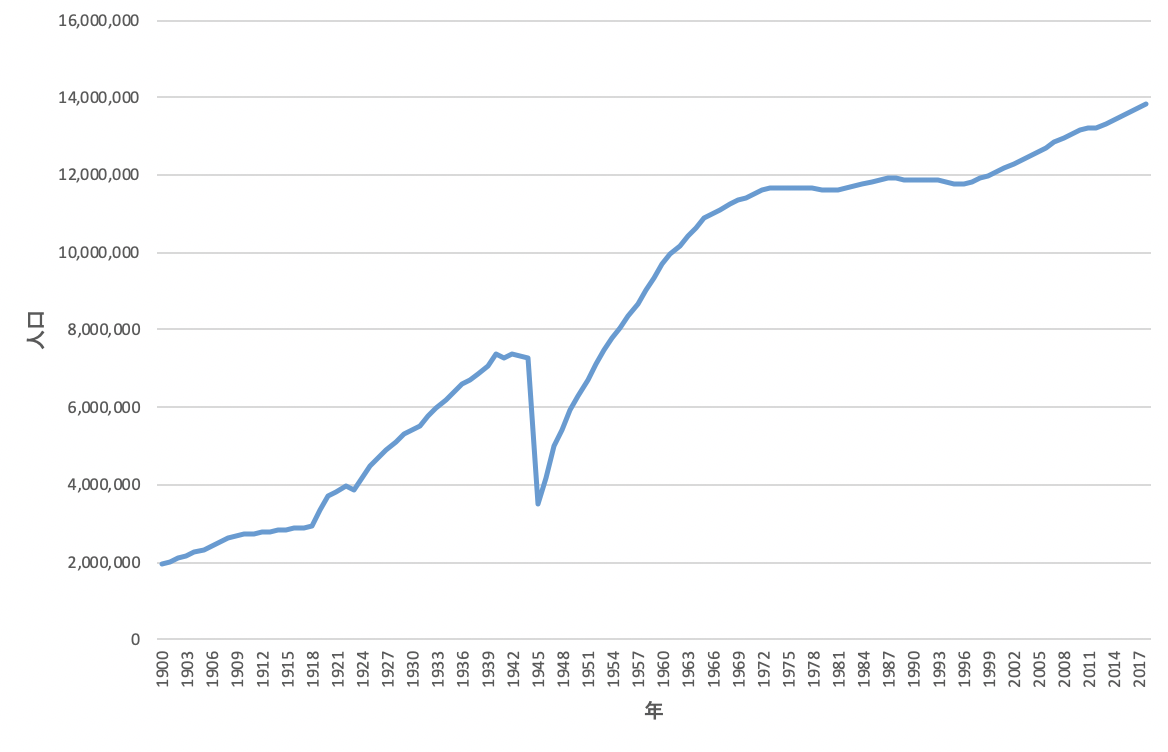
\includegraphics[scale=0.8]{kadai4_graph6.png}
    \end{center}
    \caption{東京都の人口の推移}
    \label{fig6}
\end{figure}

表3は、文献\cite{paa}より東京都の1900年から2018年の人口を示した表である。
これをもとにグラフを作成する。
時間の推移に対して人口のデータがあるので、折れ線グラフが適切であると考えた。
したがって、図6に東京都の人口の推移を折れ線グラフで示した。

図6を見るとほとんど増加傾向であるが、1945年前後で急激に低下している。
これは、日本が戦争を行っていたので、
戦死等の理由から人口が減少したと考える。
また、2000年以降に人口増加が大きいので、
経済成長により、都市部に人口が集中していると考える。
\clearpage

\section{結論}
実験で得られたデータがばらつくことを理解した。
また、データを視覚化する方法を学び、
データの要約指標のうち代表的なものを学んだ。

\section{感想}
グラフを読み取ったり考察するのは楽しかったが、
エクセルのデータをtexの表に変換する作業がとても大変だった。
% 参考文献
\begin{thebibliography}{99}
    \label{sannkoubunnkenn_chapter}
    \bibitem[1]{rikadai}東京理科大学工学部情報工学科「情報工学実験1 2020年度」
    (2020/4/6)

    \bibitem[2]{paa}東京都統計年鑑 平成30年 | 2 人口・世帯

    \url{https://www.toukei.metro.tokyo.lg.jp/tnenkan/2018/tn18q3i002.htm}

    最終閲覧日:2020/7/31

\end{thebibliography}

\appendix
%%%%%%%%%%%%%%%%%%%%%%%%%%%%%%%%%%%%%%%%%%%%%%%%%%%%%%%
\end{document}
